\documentclass[format=acmsmall, nonacm=true, review=true, screen=true]{acmart}

\usepackage[utf8]{inputenc}
\usepackage{xcolor}
\usepackage{fancyvrb}
\usepackage{minted}
\usepackage{xspace}
\usepackage{hyperref}

% Use this instead of caption to remove acmart description warnings
\newcommand{\mycaption}[1]{\Description{#1}\caption{#1}}

% Project name
\newcommand{\ltlspec}{\textit{LTLSpec}\xspace}

% For highlighting some texts
\newcommand{\red}[1]{\textcolor{red}{#1}}

% This appears to fix some font problem...
\DeclareRobustCommand{\ttfamily}{\fontencoding{T1}\fontfamily{lmtt}\selectfont}

% Junk for acmart:
\setcopyright{acmcopyright}
\copyrightyear{2021}
\acmYear{2021}
\acmDOI{N/A}
\acmBooktitle{N/A}

\title{LTLSpec: An Extensible LTL Verifier for Distributed Systems}
\subtitle{CPSC 538B Final Project Report, 2021 Winter Term 1}
\author{Eric Conlon}
\author{Yanze Li}
\author{Tarcisio Teixeira}
\authorsaddresses{}
\date{2021-12-07}

\begin{document}

\begin{abstract}
  Specifying and proving properties about distributed system is hard.
  To the best of our knowledge, there isn't a canonical way of defining distributed system models for runtime verification.
  In this project, we develop \ltlspec, a runtime verification framework which allow users to take arbitrary distributed system traces and efficiently define a formal model to specify system properties in Linear Temporal Logic (LTL).
  Our framework then provide a simple LTL verifier implementation for verifying the LTL specification regarding the formal system model.
  To address the issue that LTL is only meaning on infinite traces, we introduce a simple mechanism called \textit{truncation} that allows users to define the default behaviours of quantifiers and atomic propositions after the traces end.
  To evaluate \ltlspec, we implement three actor-based distributed system examples and their corresponding specifications. The \ltlspec can successfully verify specified properties for all three examples.
\end{abstract}

\maketitle

\section{Introduction}

Proving that a distributed system operates as intended generally requires modeling the system in a formal framework equipped with its own reasoning techniques.
At one extreme of this design space, one formally specifies the program in full in exchange for strong guarantees about its behavior in all possible executions.
At another extreme, one “merely” specifies formal properties about the observable effects of the program, only able to guarantee that these properties have not been violated in observed executions.
In this project, we propose using the latter strategy, Runtime Verification, as a relatively lightweight way to explore “responsiveness properties” of actor-based distributed systems.

We define responsiveness properties following \cite{actorservice,parthasarathy2018modular} as a kind of liveness property of the form \(\Box \forall n. (P(n) \rightarrow \Diamond Q(n))\).
As an example in plain English: “When I send a certain request, I eventually get a response to that particular request.” Propositions with this structure allow one to establish domain-specific causal relations more useful than the “happens-before” of logical time.
In general, one uses a temporal logic to express these propositions. Linear Temporal Logic (LTL), with the \textit{Always} and \textit{Eventually} operators used above, is a popular choice. However, most presentations of LTL apply it to domains only with the use of atomic predicates. One cannot express dependency between these predicates as would be necessary to encode the notion of responsiveness.

As a result, some researchers have introduced first order quantifiers for data variables \cite{khoury_automata-based_2021,margaria_execution_2016,halle_runtime_2012} in systems such as LTL-FO+.
However, in an effort to increase the usefulness and applicability of the logic, we follow a slightly different path through the design space to leave the domain of quantification abstract and not internalize equality on quantified variables.

We have built a runtime verification framework with data variable quantification, decoupled from any particular domain one would verify.
In this paper, we:
\begin{itemize}
  \item Define the \textit{theory} of a distributed system, based on the concept of a first-order logical \textit{theory} of a domain
  \item Define \textit{bridge} interfaces related to each theory that allow the verifier to quantify over data variables and verify inhabitance of atomic propositions from the domain
  \item Implement an LTL \textit{verifiers} to check axioms from the theory against monitored programs and traces
  \item Introduce the \textit{truncation} mechanism to make verification perform better and yield more meaningful results against finite traces.
  \item Evaluate the effectiveness of \ltlspec on both three distributed system examples.
\end{itemize}

\section{Background}
\subsection{Runtime Verification}
Runtime Verification (RV), sometimes also referred to as Runtime Monitoring, Trace Analysis, or Dynamic Analysis, is a lightweight formal method that, instead of exhaustively analyzing all possible program executions, only verifies the specified properties based on the current execution trace. Though limited by traces, RV can scale well and be practically integrated with existing complex systems. Moreover, it provides the most precise information regarding the current execution. Typical usage of RV includes checking the correctness of runtime behavior, detecting bugs exhibited at runtime, and enforcing runtime invariants on live systems.

Several types of monitoring methodologies are found in the current literature, \red{REF} different approaches may vary a lot in terms of interaction with the system under verification. On one extreme we have offline monitors verifying the execution trace much later it is produced whereas some online monitors may verify the trace along with the system execution. Different approaches result in different concerns, while more intrusive strategies allow early detection and even repair at runtime, offline monitors do verification at almost no overhead for the system.

Nowadays, distributed systems are ubiquitous and complex, and they suffer malfunctions for many reasons. It is desirable to monitor their correct behaviors at runtime, ensuring various safety and liveness guarantees. However, distributed systems pose new challenges to RV. The monitors need to be distributed and coordinate the distributed logs. An expressive enough specification language is also needed to describe the reactive and asynchronous nature of the system.

\subsection{LTL and LTL-FO+}
Linear Temporal Logic (LTL) is a commonly used specification language in formal methods to express properties in reactive and concurrent systems. The basic building blocks for LTL are called atomic propositions, which are opaque, domain-specific symbols (like $P$ or $Q$). Atomic propositions can then be connected or negate with standard boolean operators, including $\land$ (and), $\lor$ (or), $\lnot$ (not), and $\Rightarrow$ (implies), following their classical logic meaning. Most importantly, LTL introduces a set of temporal operators. Let $\phi$ be a proposition:
\begin{itemize}
  \item Operator $\Box$ means  ``always'', $\Box \phi$ means that $\phi$ is true in \textit{every} future time step.
  \item Operator $\Diamond$ means ``eventually'', $\Diamond \phi$ means that $\phi$ holds for \textit{some} future time steps.
  \item Operator $\bigcirc$ means ``next'', $\bigcirc \phi$ means that $\phi$ holds for the \textit{next} time step.
  \item Operator $\mathcal{U}$ means ``Until'', $\phi \mathcal{U}\psi$ means that $\phi$ holds for all time steps until at some step $\psi$ holds. $\psi$ must hold at the current step or in the future.
  \item Operator $\mathcal{W}$ means ``Weak Until'', $\phi \mathcal{W}\psi$ means that $\phi$ holds for all time steps until at some step $\psi$ holds. If $\psi$ never holds, then $\phi$ must hold forever.
\end{itemize}

To achieve stronger expressiveness, different extensions of LTL are proposed. Early work by Emerson [7] extended LTL with standard first order quantifiers, where the variables are quantified over a fixed domain. A different approach, inspired by the database community, quantifies the variables over a dynamic domain, i.e., variables appear in the trace. The latter is more favorable for RV, since the dynamic domain is more tractable algorithmically. Hence, in our project, we decided to use an LTL extension called LTL-FO+.

LTL-FO+ allows users to quantify over the values seen at the current time step. Given a parameter identifier $p$ and a proposition $\phi$, then $\exists_{p} x : \phi$ and $\forall_{p} x:\phi$ are also propositions. Assume $\rho$ is the trace of the system at the current time, then the semantics of the quantifiers can be formalized as below:

$$\rho\vDash \exists_p x:\phi \Leftrightarrow \phi[b/x] \text{for some }b\in Dom_{\rho}(p)$$
$$\forall_{p} x : \phi \equiv \lnot(\exists_{p}x: \lnot\phi)$$

Note that the domain whose we quantify over is a function of the parameter identifier and the trace at the current time.

For example, let's assume that one wants to check if the property “At some point in the system there exists one messageId with value $v$ such that some atomic proposition $\phi(v)$ holds” is satisfied at the current time. Then, using LTL-FO+ we would write the above as follows:

$$ \rho \vDash \Diamond(\exists_{p} v :\phi(v)) $$


The quantifier in LTL-FO+ only quantifies over data variables, therefore it cannot express propositions that quantifies over time. Since it is based on first order logic, it also disallows user to quantify over things like properties.

\section{LTLSpec}

\begin{figure}[h]
  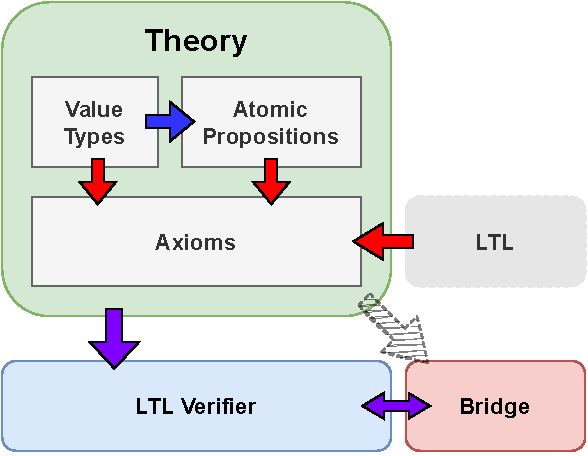
\includegraphics[width=0.6\textwidth]{images/ltlspec-overview.pdf}
  \centering
  \caption{Overview of LTLSpec}
  \label{fig:overview}
\end{figure}

\ltlspec is a verification framework aiming at providing a canonical way for specifying arbitrary LTL properties in distributed system.
Figure~\ref{fig:overview} shows the overview of the framework.
At a high level, \ltlspec consists of three components.
The \textit{theory} is a user-defined domain for verification that includes the definitions of \textit{value types}, \textit{atomic propositions}, and \textit{axioms} about the system.
The \textit{bridge} defines how to evaluate quantifiers over value types and atomic propositions in the axioms.
The LTL verifier is an interpreter over the LTL abstract syntax tree.
The details about the components will be further explained in the following subsections, along with our extension to the bridge, namely \textit{truncation}.

The verification is performed over a trace, where each element inside is called a \textit{world}.
Each axiom is verified against a world. The LTL verifier is in charge of interpreting the LTL connectives.
Once the verifier hits a quantifier or atomic proposition, it passes the current world and the corresponding quantifier or proposition to the bridge for evaluation.
This interaction ends until the axiom can no longer be evaluated.
Since proposition written in LTL talks about system properties spanning multiple worlds, the residual of the current evaluation will be carried along for further evaluation in the next world.


\subsection{First-order theories}
\label{subsec:theory}

\red{
  First, we will loosely define a language for expressing the \textit{theory} of a user’s domain.
  DFOL (First Order Logic with Dependent types) as encoded in LF syntax \cite{hutchison_first-order_2006} is an excellent fit for this task. It allows one to define the types of values in a domain, as well as atomic propositions over those values. (This is called a \textit{signature}.)
  Additionally, it allows one to express propositions with quantifiers or \textit{axioms}. Together, the signature and axioms form a theory of the domain.
}

\begin{figure}[h]
  {
    \fontsize{10}{12}\selectfont
    \begin{Verbatim}[commandchars=\\\{\},codes={\catcode`$=3}]
\textcolor{black}{(*} \textcolor{black}{A ping request sent by an actor} \textcolor{black}{*)}
\textcolor{blue}{SentPing} \textcolor{darkgray}{:} \textcolor{cyan}{Set}
\textcolor{black}{(*} \textcolor{black}{A pong response received by an actor} \textcolor{black}{*)}
\textcolor{blue}{RecvPong} \textcolor{darkgray}{:} \textcolor{cyan}{Set}

\textcolor{black}{(*} \textcolor{black}{Characterizes a request-response pair} \textcolor{black}{*)}
\textcolor{teal}{IsPingPong} \textcolor{darkgray}{:} \textcolor{blue}{SentPing} \textcolor{darkgray}{$\rightarrow$} \textcolor{blue}{RecvPong} \textcolor{darkgray}{$\rightarrow$} \textcolor{cyan}{Prop}

\textcolor{black}{(*} \textcolor{black}{Every ping request eventually gets a pong response} \textcolor{black}{*)}
\textcolor{purple}{isResponsive} \textcolor{darkgray}{:} 
  \textcolor{teal}{$\Box$} \textcolor{darkgray}{(}\textcolor{teal}{$\forall$} \textcolor{darkgray}{(}\textcolor{red}{m1} \textcolor{darkgray}{:} \textcolor{blue}{SentPing}\textcolor{darkgray}{)}\textcolor{darkgray}{,} 
    \textcolor{teal}{$\Diamond$} \textcolor{darkgray}{(}\textcolor{teal}{$\exists$} \textcolor{darkgray}{(}\textcolor{red}{m2} \textcolor{darkgray}{:} \textcolor{blue}{RecvPong}\textcolor{darkgray}{)}\textcolor{darkgray}{,} 
      \textcolor{teal}{IsPingPong} \textcolor{purple}{m1} \textcolor{purple}{m2}\textcolor{darkgray}{)}\textcolor{darkgray}{)}
\end{Verbatim}

  }
  \mycaption{Theory for a trivial ping system}
  \label{fig:ping-theory}
\end{figure}

\subsection{Bridge}
\label{subsec:bridge}

The theory provides a set of interfaces restricting what types, propositions, and invariants we can talk about regarding a specific distributed system trace, yet it does not provide an interpretation about for propositions and quantifiers over types.
The bridge is the component answering those questions.

\begin{figure}[h]
  {
    \fontsize{10}{12}\selectfont
    \begin{minted}{haskell}
class Eq v => Bridge e v w | w -> e v where
  -- Evaluate the atomic proposition or fail.
  bridgeEvalProp :: w -> Atom v -> Either e Prop
  -- Quantify over all values of the given type or fail.
  bridgeQuantify :: w -> TyName -> Either e [v]
\end{minted}
  }
  \mycaption{Haskell definition of a bridge}
  \label{fig:bridge-sig}
\end{figure}

Figure~\ref{fig:bridge-sig} presents the typeclass definition for bridges.
Two functions \texttt{bridgeEvalProp} and \texttt{bridgeQuantify} needs to be implemented.
\texttt{bridgeEvalProp} decides how to evaluate an atomic proposition when given correct inputs. It takes the current world \texttt{w} and the atomic proposition \texttt{Atom v} of interest as arguments.
It either returns an error message \texttt{e}, if the proposition could not be successfully evaluated, or a resulting proposition \texttt{Prop} if the evaluation succeeded.
For most bridge definitions, the value of \texttt{Prop} here should be either one of the constants between \texttt{PropTrue} and \texttt{PropFalse}.

\texttt{bridgeQuantify} decides how to quantify over a specific type name regarding the current world.
Similarly, it takes the current world \texttt{w} and a type name as arguments, and produce either an error \texttt{e} or a list of values \texttt{v} of the given type for quantification results.

In our current implementation, there isn't a mechanism to guarantee the correspondence between the theory and the bridge, and it is users' responsibility to make sure all types and propositions are correctly quantified or evaluated in the brdige.
It is possible to provide users with a surface language where the compiler guarantees all bridge definitions respects the theory of the distributed system. We consider this as a future work.

\subsection{Verifier}

The verifier is an interpreter over the abstract syntax tree of an LTL proposition. Figure~\ref{fig:verifier-sig} gives the data type definition of \texttt{EnvProp} and the signature of the evaluation function \texttt{envPropEval}.

\begin{figure}[h]
  {
    \fontsize{10}{12}\selectfont
    \begin{minted}{haskell}
-- EnvProp is an LTL proposition with its environment
-- The environment carries the data variable v
-- introduced by quantifiers in the parent propositions.
data EnvProp v =
  EnvProp !(Env v) !Prop
-- Evaluate LTL Proposition
envPropEval :: Bridge e v w => EnvProp v -> w -> EnvPropRes e v
\end{minted}
  }
  \mycaption{Haskell definition of the data type \texttt{EnvProp} and the evaluation function}
  \label{fig:verifier-sig}
\end{figure}

\texttt{EnvProp} is a wrapper for primitive LTL propositions \texttt{Prop}.
It carries an additional field \texttt{Env v} that keeps track of the variable bindings introduced by quantifiers in the parent propositions.

To evaluate an LTL proposition, \texttt{envPropEval} takes an \texttt{EnvProp} and the current world \texttt{w} to compute a resulting proposition \texttt{EnvPropRes}.
The result can be a boolean value, when a proposition is fully evaluated in the current world.
If the proposition involves modal connectives that cannot be evaluated immediate, the function returns a residual proposition that will be carried along to the next world.
If the proposition involves any quantifiers or atomic propositions, the evaluator will invoke the corresponding bridge functions explained in section~\ref{subsec:bridge} using the current world \texttt{w}.

The \texttt{envPropEval} only evaluate the LTL proposition on a single world, i.e., one element in the distributed system trace.
To fully verify the system, we call \texttt{envPropEval} iteratively over an entire system trace.
At each iteration \texttt{envPropEval} take the residual proposition from last one together with the current world as arguments.
The verification process stops when either the proposition is evaluated to be true or false, the whole trace is consumed, or the evaluator throws an exception.

It is worth noticing that our implementation does not assume a specific way of doing the verification.
Users can easily integrate the verifier with either a pre-collected trace (offline verification) or a running system actively generating new traces (online verification).

\subsection{Truncation}

One issue for all LTL-based runtime verification technique is that modal connectives are only meaningful regarding infinite traces.
Taking the ping-pong system in section~\ref{subsec:theory} for example, the axiom (invariant) we want the system to hold is \texttt{isResponsive}.
This proposition start with the modal connective ``$\Diamond$ (always)'', meaning the proposition needs to hold in \textit{all} future executions.
However, in practice we can only do runtime verification on finite traces, thus this proposition can never be proven true but only disproven when a violation is detected.

Such behaviour is not always desirable when a system has been monitored for sufficiently long and certain assumptions can be made for its future executions.
To allow users to make assumptions for their systems' behaviors \textit{after} the current traces, we provide a mechanism called \textit{truncation}.

The definition of truncation is essentially an extension to the bridge, as shown in figure~\ref{fig:truncation-sig}.

\begin{figure}[h]
  {
    \fontsize{10}{12}\selectfont
    \begin{minted}{haskell}
-- A 'Bridge' that supports proposition truncation.
class Bridge e v w => TruncBridge e v w where
  -- The set of types with empty quantification in *all reachable worlds*
  truncBridgeEmpty :: w -> Set TyName
  -- An oracle for atomic propositions in *all reachable worlds*
  truncBridgeOracle :: w -> Atom v -> Either e TriBool
\end{minted}
  }
  \mycaption{Haskell definition of a truncation bridge}
  \label{fig:truncation-sig}
\end{figure}

Similar to bridges, users need to implement two functions that talks about quantifications and atomic propositions respectively.
\texttt{truncBridgeEmpty} takes the last world in the trace, and decides which set of types have empty quantification.
\texttt{truncBridgeOracle} evaluates atomic propositions based on the last world.

As a result, all propositions will be truncated into a ternary value, namely \textit{true}, \textit{false}, or \textit{unknown}.
For example, propositions that are universally (existentially) quantified over these truncated types will be evaluated to be true (false) while the rest being unknown.
An unknown proposition preserves the original LTL semantics, meaning it is not violated up to the point the monitoring ends, but it remains unknown whether the proposition holds in the future.

\section{Evaluation}

We evaluate our \ltlspec by verifying three simple distributed systems, i.e. a ping-pong system, a chat room implementation, and an implementation of the dinning philosopher problem.

\subsection{Implementation}

The \ltlspec framework, all example systems, and the corresponding theories and bridges are implemented in Haskell.
We use software transactional memory (STM) to implement the tracing to preserve the causality of the entire traces.
The project is open-sourced and can be found \href{https://github.com/ejconlon/ltlspec}{here}

\subsection{Ping-Pong}

\subsection{Chat Room}
\begin{figure}[ht]
  {
    \fontsize{10}{12}\selectfont
    \begin{Verbatim}[commandchars=\\\{\},codes={\catcode`$=3},fontsize=\small]
\textcolor{blue}{Client} \textcolor{darkgray}{:} \textcolor{cyan}{Set}
\textcolor{blue}{Channel} \textcolor{darkgray}{:} \textcolor{cyan}{Set}
\textcolor{blue}{Action} \textcolor{darkgray}{:} \textcolor{cyan}{Set}


\textcolor{teal}{ChannelListNote} \textcolor{darkgray}{:} \textcolor{blue}{Action} \textcolor{darkgray}{$\rightarrow$} \textcolor{blue}{Client} \textcolor{darkgray}{$\rightarrow$} \textcolor{blue}{Channel} \textcolor{darkgray}{$\rightarrow$} \textcolor{cyan}{Prop}
\textcolor{teal}{IsMember} \textcolor{darkgray}{:} \textcolor{blue}{Client} \textcolor{darkgray}{$\rightarrow$} \textcolor{blue}{Channel} \textcolor{darkgray}{$\rightarrow$} \textcolor{cyan}{Prop}
\textcolor{teal}{IsSameClient} \textcolor{darkgray}{:} \textcolor{blue}{Client} \textcolor{darkgray}{$\rightarrow$} \textcolor{blue}{Client} \textcolor{darkgray}{$\rightarrow$} \textcolor{cyan}{Prop}
\textcolor{teal}{Joined} \textcolor{darkgray}{:} \textcolor{blue}{Action} \textcolor{darkgray}{$\rightarrow$} \textcolor{blue}{Client} \textcolor{darkgray}{$\rightarrow$} \textcolor{blue}{Channel} \textcolor{darkgray}{$\rightarrow$} \textcolor{cyan}{Prop}
\textcolor{teal}{Left} \textcolor{darkgray}{:} \textcolor{blue}{Action} \textcolor{darkgray}{$\rightarrow$} \textcolor{blue}{Client} \textcolor{darkgray}{$\rightarrow$} \textcolor{blue}{Channel} \textcolor{darkgray}{$\rightarrow$} \textcolor{cyan}{Prop}
\textcolor{teal}{ListRequested} \textcolor{darkgray}{:} \textcolor{blue}{Action} \textcolor{darkgray}{$\rightarrow$} \textcolor{blue}{Client} \textcolor{darkgray}{$\rightarrow$} \textcolor{cyan}{Prop}
\textcolor{teal}{NewJoinNote} \textcolor{darkgray}{:} \textcolor{blue}{Action} \textcolor{darkgray}{$\rightarrow$} \textcolor{blue}{Client} \textcolor{darkgray}{$\rightarrow$} \textcolor{blue}{Channel} \textcolor{darkgray}{$\rightarrow$} \textcolor{blue}{Client} \textcolor{darkgray}{$\rightarrow$} \textcolor{cyan}{Prop}
\textcolor{teal}{NewLeaveNote} \textcolor{darkgray}{:} \textcolor{blue}{Action} \textcolor{darkgray}{$\rightarrow$} \textcolor{blue}{Client} \textcolor{darkgray}{$\rightarrow$} \textcolor{blue}{Channel} \textcolor{darkgray}{$\rightarrow$} \textcolor{blue}{Client} \textcolor{darkgray}{$\rightarrow$} \textcolor{cyan}{Prop}
\textcolor{teal}{Sent} \textcolor{darkgray}{:} \textcolor{blue}{Action} \textcolor{darkgray}{$\rightarrow$} \textcolor{blue}{Client} \textcolor{darkgray}{$\rightarrow$} \textcolor{blue}{Channel} \textcolor{darkgray}{$\rightarrow$} \textcolor{cyan}{Prop}
\textcolor{teal}{Shared} \textcolor{darkgray}{:} \textcolor{blue}{Action} \textcolor{darkgray}{$\rightarrow$} \textcolor{blue}{Client} \textcolor{darkgray}{$\rightarrow$} \textcolor{blue}{Client} \textcolor{darkgray}{$\rightarrow$} \textcolor{cyan}{Prop}


\textcolor{purple}{ifInChannelReceiveMessage} \textcolor{darkgray}{:} 
  \textcolor{teal}{$\Box$} \textcolor{darkgray}{(}\textcolor{teal}{$\forall$} \textcolor{darkgray}{(}\textcolor{red}{c1} \textcolor{red}{c2} \textcolor{darkgray}{:} \textcolor{blue}{Client}\textcolor{darkgray}{)} \textcolor{darkgray}{(}\textcolor{red}{ch} \textcolor{darkgray}{:} \textcolor{blue}{Channel}\textcolor{darkgray}{)} \textcolor{darkgray}{(}\textcolor{red}{m} \textcolor{darkgray}{:} \textcolor{blue}{Action}\textcolor{darkgray}{)}\textcolor{darkgray}{,} 
    \textcolor{darkgray}{(}\textcolor{darkgray}{(}\textcolor{teal}{$\neg$} \textcolor{darkgray}{(}\textcolor{teal}{IsSameClient} \textcolor{purple}{c1} \textcolor{purple}{c2}\textcolor{darkgray}{)}\textcolor{darkgray}{)} \textcolor{teal}{$\land$} \textcolor{darkgray}{(}\textcolor{teal}{IsMember} \textcolor{purple}{c1} \textcolor{purple}{ch}\textcolor{darkgray}{)} \textcolor{teal}{$\land$} \textcolor{darkgray}{(}\textcolor{teal}{IsMember} \textcolor{purple}{c2} \textcolor{purple}{ch}\textcolor{darkgray}{)} \textcolor{teal}{$\land$} \textcolor{darkgray}{(}\textcolor{teal}{Sent} \textcolor{purple}{m} \textcolor{purple}{c1} \textcolor{purple}{ch}\textcolor{darkgray}{)}\textcolor{darkgray}{)} \textcolor{teal}{$\implies$} \textcolor{darkgray}{(}\textcolor{teal}{$\Diamond$} \textcolor{darkgray}{(}\textcolor{teal}{Shared} \textcolor{purple}{m} \textcolor{purple}{c1} \textcolor{purple}{c2}\textcolor{darkgray}{)}\textcolor{darkgray}{)}\textcolor{darkgray}{)}
\textcolor{purple}{isMemberBetweenJoinAndLeave} \textcolor{darkgray}{:} 
  \textcolor{teal}{$\Box$} \textcolor{darkgray}{(}\textcolor{teal}{$\forall$} \textcolor{darkgray}{(}\textcolor{red}{c} \textcolor{darkgray}{:} \textcolor{blue}{Client}\textcolor{darkgray}{)} \textcolor{darkgray}{(}\textcolor{red}{ch} \textcolor{darkgray}{:} \textcolor{blue}{Channel}\textcolor{darkgray}{)}\textcolor{darkgray}{,} 
    \textcolor{teal}{$\exists$} \textcolor{darkgray}{(}\textcolor{red}{i} \textcolor{red}{j} \textcolor{darkgray}{:} \textcolor{blue}{Action}\textcolor{darkgray}{)}\textcolor{darkgray}{,} 
      \textcolor{darkgray}{(}\textcolor{teal}{Joined} \textcolor{purple}{i} \textcolor{purple}{c} \textcolor{purple}{ch}\textcolor{darkgray}{)} \textcolor{teal}{$\implies$} \textcolor{darkgray}{(}\textcolor{teal}{U} \textcolor{darkgray}{(}\textcolor{teal}{IsMember} \textcolor{purple}{c} \textcolor{purple}{ch}\textcolor{darkgray}{)} \textcolor{darkgray}{(}\textcolor{teal}{Left} \textcolor{purple}{j} \textcolor{purple}{c} \textcolor{purple}{ch}\textcolor{darkgray}{)}\textcolor{darkgray}{)}\textcolor{darkgray}{)}
\textcolor{purple}{neverSendMessageToMyself} \textcolor{darkgray}{:} 
  \textcolor{teal}{$\Box$} \textcolor{darkgray}{(}\textcolor{teal}{$\forall$} \textcolor{darkgray}{(}\textcolor{red}{c} \textcolor{darkgray}{:} \textcolor{blue}{Client}\textcolor{darkgray}{)} \textcolor{darkgray}{(}\textcolor{red}{m} \textcolor{darkgray}{:} \textcolor{blue}{Action}\textcolor{darkgray}{)}\textcolor{darkgray}{,} 
    \textcolor{teal}{$\neg$} \textcolor{darkgray}{(}\textcolor{teal}{Shared} \textcolor{purple}{m} \textcolor{purple}{c} \textcolor{purple}{c}\textcolor{darkgray}{)}\textcolor{darkgray}{)}
\end{Verbatim}

  }
  \mycaption{Theory for a chat room system}
  \label{fig:chat-theory}
\end{figure}

\subsection{Dinning Philosopher}
\begin{figure}[ht]
  {
    \fontsize{10}{12}\selectfont
    \begin{Verbatim}[commandchars=\\\{\},codes={\catcode`$=3}]
\textcolor{black}{(*} \textcolor{black}{The id of an actor representing a hakker (philosopher)} \textcolor{black}{*)}
\textcolor{blue}{Hakker} \textcolor{darkgray}{:} \textcolor{cyan}{Set}
\textcolor{black}{(*} \textcolor{black}{The id of an actor representing a chopstick} \textcolor{black}{*)}
\textcolor{blue}{Chopstick} \textcolor{darkgray}{:} \textcolor{cyan}{Set}
\textcolor{black}{(*} \textcolor{black}{A message sent by a hakker} \textcolor{black}{*)}
\textcolor{blue}{HakkerMsg} \textcolor{darkgray}{:} \textcolor{cyan}{Set}
\textcolor{black}{(*} \textcolor{black}{A message sent by a chopstick} \textcolor{black}{*)}
\textcolor{blue}{ChopstickMsg} \textcolor{darkgray}{:} \textcolor{cyan}{Set}


\textcolor{teal}{FromAdjacent} \textcolor{darkgray}{:} \textcolor{blue}{Chopstick} \textcolor{darkgray}{$\rightarrow$} \textcolor{blue}{HakkerMsg} \textcolor{darkgray}{$\rightarrow$} \textcolor{cyan}{Prop}
\textcolor{teal}{InitiallyThinking} \textcolor{darkgray}{:} \textcolor{blue}{Hakker} \textcolor{darkgray}{$\rightarrow$} \textcolor{cyan}{Prop}
\textcolor{teal}{IsEating} \textcolor{darkgray}{:} \textcolor{blue}{Hakker} \textcolor{darkgray}{$\rightarrow$} \textcolor{cyan}{Prop}
\textcolor{teal}{IsHungry} \textcolor{darkgray}{:} \textcolor{blue}{Hakker} \textcolor{darkgray}{$\rightarrow$} \textcolor{cyan}{Prop}
\textcolor{teal}{ReceivedNotDelivered} \textcolor{darkgray}{:} \textcolor{blue}{Chopstick} \textcolor{darkgray}{$\rightarrow$} \textcolor{blue}{HakkerMsg} \textcolor{darkgray}{$\rightarrow$} \textcolor{cyan}{Prop}


\textcolor{black}{(*} \textcolor{black}{All hakkers that are initially thinking should eventually start eating} \textcolor{black}{*)}
\textcolor{purple}{liveness} \textcolor{darkgray}{:} 
  \textcolor{teal}{$\Box$} \textcolor{darkgray}{(}\textcolor{teal}{$\forall$} \textcolor{darkgray}{(}\textcolor{red}{h} \textcolor{darkgray}{:} \textcolor{blue}{Hakker}\textcolor{darkgray}{)}\textcolor{darkgray}{,} 
    \textcolor{darkgray}{(}\textcolor{teal}{InitiallyThinking} \textcolor{purple}{h}\textcolor{darkgray}{)} \textcolor{teal}{$\implies$} \textcolor{darkgray}{(}\textcolor{teal}{$\Diamond$} \textcolor{darkgray}{(}\textcolor{teal}{IsEating} \textcolor{purple}{h}\textcolor{darkgray}{)}\textcolor{darkgray}{)}\textcolor{darkgray}{)}
\textcolor{black}{(*} \textcolor{black}{All messages a chopstick received come from its adjacent hakkers} \textcolor{black}{*)}
\textcolor{purple}{receiveFromAdjacentHakkers} \textcolor{darkgray}{:} 
  \textcolor{teal}{$\Box$} \textcolor{darkgray}{(}\textcolor{teal}{$\forall$} \textcolor{darkgray}{(}\textcolor{red}{c} \textcolor{darkgray}{:} \textcolor{blue}{Chopstick}\textcolor{darkgray}{)} \textcolor{darkgray}{(}\textcolor{red}{hm} \textcolor{darkgray}{:} \textcolor{blue}{HakkerMsg}\textcolor{darkgray}{)}\textcolor{darkgray}{,} 
    \textcolor{darkgray}{(}\textcolor{teal}{ReceivedNotDelivered} \textcolor{purple}{c} \textcolor{purple}{hm}\textcolor{darkgray}{)} \textcolor{teal}{$\implies$} \textcolor{darkgray}{(}\textcolor{teal}{FromAdjacent} \textcolor{purple}{c} \textcolor{purple}{hm}\textcolor{darkgray}{)}\textcolor{darkgray}{)}
\end{Verbatim}

  }
  \mycaption{Theory for the dinning philosopher problem}
  \label{fig:phil-theory}
\end{figure}

\section{Related Work}

Previous work has developed logical frameworks extending separation logic to specify the responsiveness properties in actor-based systems and do proofs in Hoare-Logic style \cite{actorservice, parthasarathy2018modular}.
However, these logical frameworks have yet proven to be practical nor integrated into some existing program verification tools.
On the other hand, there are only limited existing works adopting RV for actor-based systems.
Some existing works \cite{shafiei2020actor,lavery2017actor} use the actor model to implement RV tools.
The most relevant works we can find are \cite{cassar2015synchronous,cassar2015runtime}.
\cite{cassar2015synchronous} studied the overhead between synchronous and asynchronous monitor instrumentation for actor-based systems and proposed a hybrid instrumentation technique that can be  integrated with RV tools to provide timely detection with low runtime overhead.
\cite{cassar2015runtime} proposed a runtime adaptation technique based on an existing RV tool to dynamically react to violations detected in actor-based systems.
In our project, instead of focusing on the RV techniques specifically for actor-based systems, we emphasize on how to provide an abstraction layer between the distributed application and the LTL verifiers.
We want to provide an expressive specification language to help users model their application domains and specify the system's properties at the same time. This specification later acts as the contract between the real system and the verifier.
We pick the actor-based system because it's a popular programming model and a clean abstraction for distributed systems.
Previous work has also shown that interesting properties about actor-based systems can be specified using an LTL-like logic[1,5].

\section{Conclusion}

TODO.

\pagebreak

\bibliographystyle{ACM-Reference-Format}
\bibliography{ltlspec-report}

\end{document}
